\begin{figure*}[t]
\centering
% Vector drawing generated by tools/figures/lifecycle.py; rerun it after changing the figure.
\ifbilingual
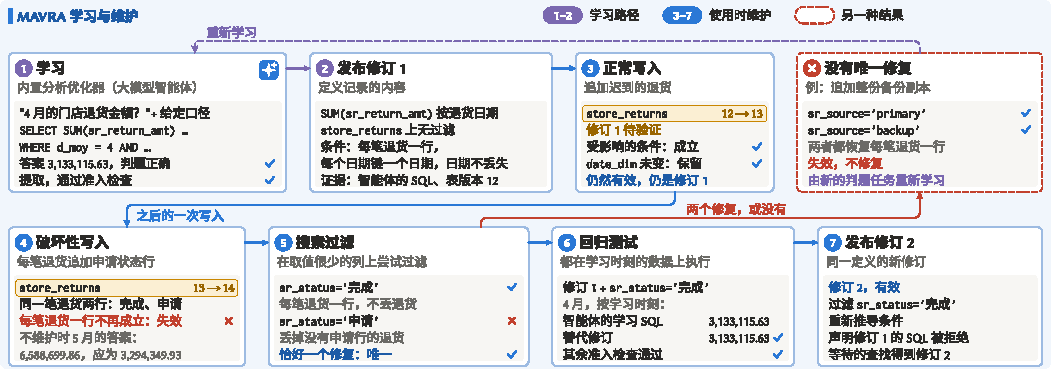
\includegraphics[width=\textwidth]{figures/lifecycle-zh}
\else
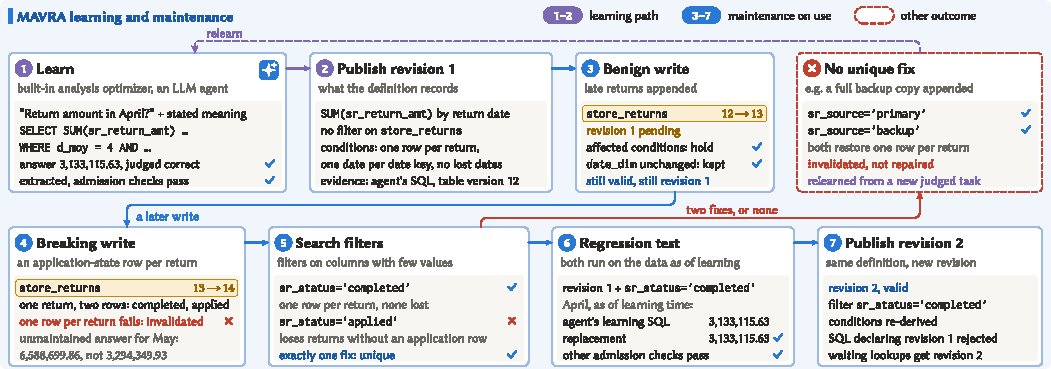
\includegraphics[width=\textwidth]{figures/lifecycle}
\fi
\caption{\bt{Learning and maintenance of one definition. A benign write keeps the revision (3); a breaking write invalidates it (4), and bounded repair publishes a replacement only if exactly one filter restores one row per return (5) and, as of learning time, reproduces the agent's learning answer (6). Otherwise (red) the definition stays unavailable until it is relearned.}{一个定义的学习与维护。正常写入后修订不变（3）；破坏性写入使其失效（4），有界修复只在恰好一个过滤能恢复每笔退货一行（5）且按学习时刻复现智能体的学习答案（6）时发布替代修订。否则（红框）定义在重新学习之前不可用。}}
\label{fig:lifecycle}
\Description{Two rows of steps with example values. Top row: step 1, learn: the built-in analysis optimizer, an LLM agent, answers ``Return amount in April?'' with a stated meaning, using SQL that sums sr\_return\_amt for month 4; the answer 3,133,115.63 is judged correct, extracted, and passes admission. Step 2 publishes revision 1: SUM(sr\_return\_amt) by return date, no filter, the conditions one row per return, one date per date key, and no lost dates, and as evidence the agent's SQL and table version 12. Step 3, a benign write of late returns, moves store\_returns from 12 to 13; revision 1 is pending, the affected conditions are rechecked and hold, the date\_dim result is kept, and revision 1 stays valid. Bottom row: step 4, a breaking write adding an application-state row per return, moves store\_returns from 13 to 14; one return now has a completed and an applied row, one row per return fails, and revision 1 is invalidated; unmaintained, the May answer would be 6,588,699.86 instead of 3,294,349.93. Step 5 searches filters on columns with few values: sr\_status = 'completed' keeps one row per return and loses none, sr\_status = 'applied' loses returns without an application row, so exactly one fix exists. Step 6, the regression test on the data as of learning time, gives 3,133,115.63 for both the agent's learning SQL and the replacement, which also passes the other admission checks. Step 7 publishes revision 2 with the filter, re-derives the conditions, rejects SQL that declares revision 1, and gives waiting lookups revision 2. A red dashed box on the top right shows the other outcome: after a full backup copy, sr\_source = 'primary' and sr\_source = 'backup' both restore one row per return, so the definition is invalidated, not repaired, and a dashed violet arrow returns to step 1 to relearn it from a new judged task.}
\end{figure*}
